\documentclass[11pt]{article}
\usepackage[utf8]{inputenc}
\usepackage[T1]{fontenc}
\usepackage{minted}
\usepackage{graphicx}
\usepackage{hyperref}

\author{Student: Sean Wang, szw87 \\ Professor: Mohit Tiwari, Antonio Espinoza \\ Department of Electrical \& Computer Engineering \\ The University of Texas at Austin}
\date{\today}
\title{EE379K Enterprise Network Security Lab 2 Report}
\hypersetup{
 pdfauthor={Student: Sean Wang, szw87 \\ Professor: Mohit Tiwari, Antonio Espinoza \\ Department of Electrical \& Computer Engineering \\ The University of Texas at Austin},
 pdftitle={EE379K Enterprise Network Security Lab 2 Report},
 pdfkeywords={},
 pdfsubject={},
 pdfcreator={},
 pdflang={English}}

\begin{document}

\maketitle
\section*{Part 3 - Orchestration}
\subsection*{3a - Orchestration with Kubernetes}
\subsubsection*{Docker applications}
Running the simple PHP and MySQL server example with
\begin{minted}{bash}
  $ docker-compose up
\end{minted}
sets up both the web-service and SQL DB are on localhost. The web-service can be accessed through \verb|localhost:8000|,
which maps internally to port 80 inside the container. Additionally, the web-service uses port 3306 to access the SQL DB,
while port 8082 is exposed to the host. The contents seen on the homepage, \verb|http://localhost:8000|, is due to
\verb|src/index.php|. \\
By going into \verb|docker-compose.yml| and changing the port mapping from \verb|8000:80| to \verb|9000:80|, as shown in
Figure~\ref{fig:port}, the web-server can now be accessed at \verb|http://localhost:9000|, since this changed what port is
exposed to the host machine and maps it to the internal port.
\clearpage
\begin{figure}[h!]
  \centering
  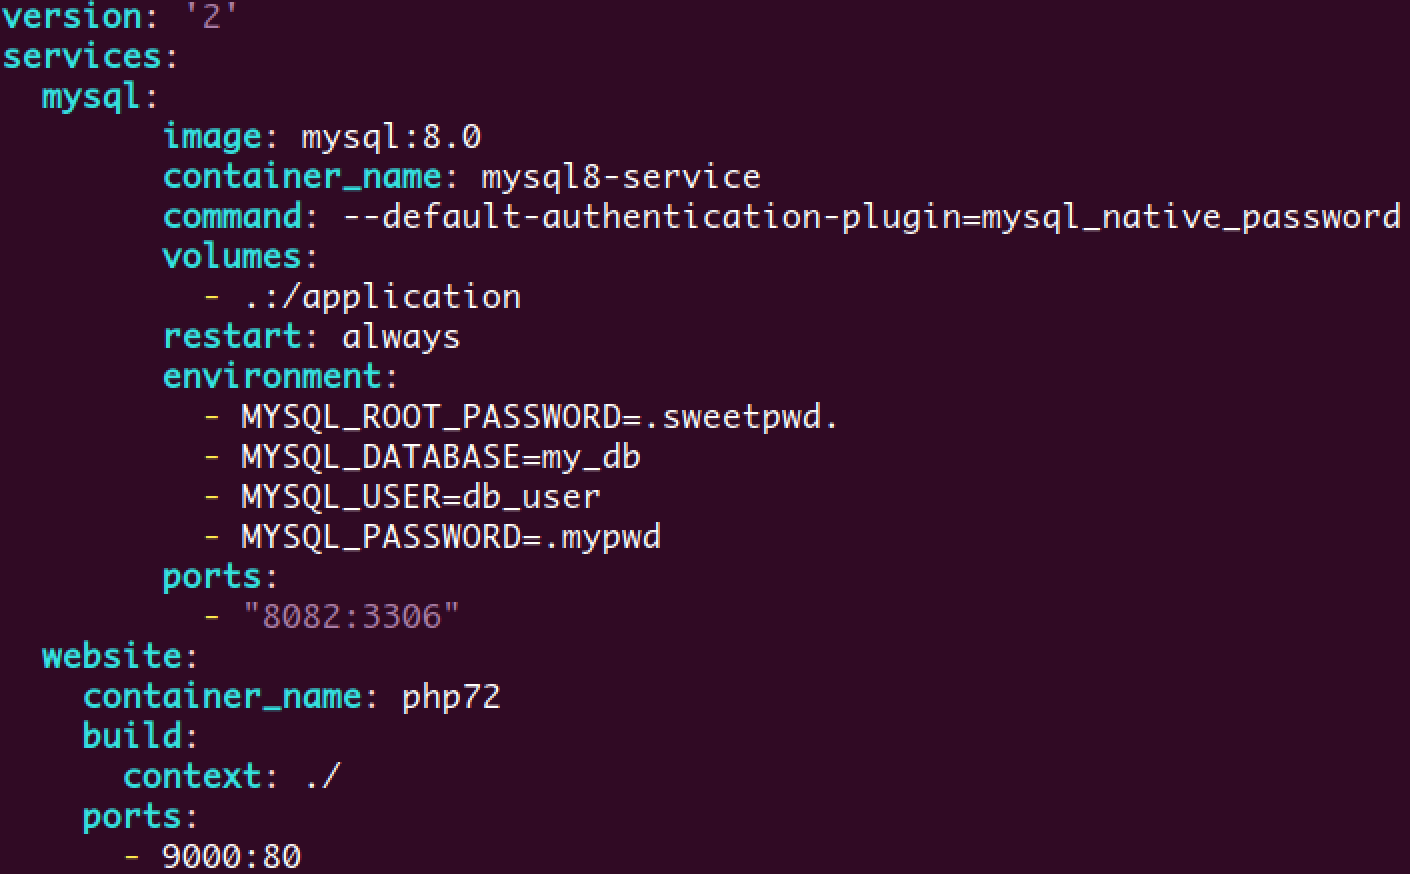
\includegraphics[width=1\linewidth]{./docker_port.png}
  \caption{\label{fig:port}
  Changing port mapping inside docker-compose.yml}
\end{figure}
\subsubsection*{Kubernetes}
After tagging and pushing the web-service image to the microk8s registry, then the following commands are used to run the
web-application in kubernetes:
\begin{minted}{bash}
  $ microk8s.kubectl apply -f webserver.yaml
  $ microk8s.kubectl apply -f webserver-svc.yaml
  $ microk8s.kubectl apply -f mysql.yaml
  $ microk8s.kubectl apply -f mysql-svc.yaml
\end{minted}
Then, the different namespaces, shown in Figure~\ref{fig:pods} and Figure~\ref{fig:svcs}, are seen under the
\verb|NAMESPACE| column in each of the outputs of the following commands:
\begin{minted}{bash}
  $ microk8s.kubectl get pods --all-namespaces
  $ microk8s.kubectl get services --all-namespaces
\end{minted}
\begin{figure}[htbp]
  \centering
  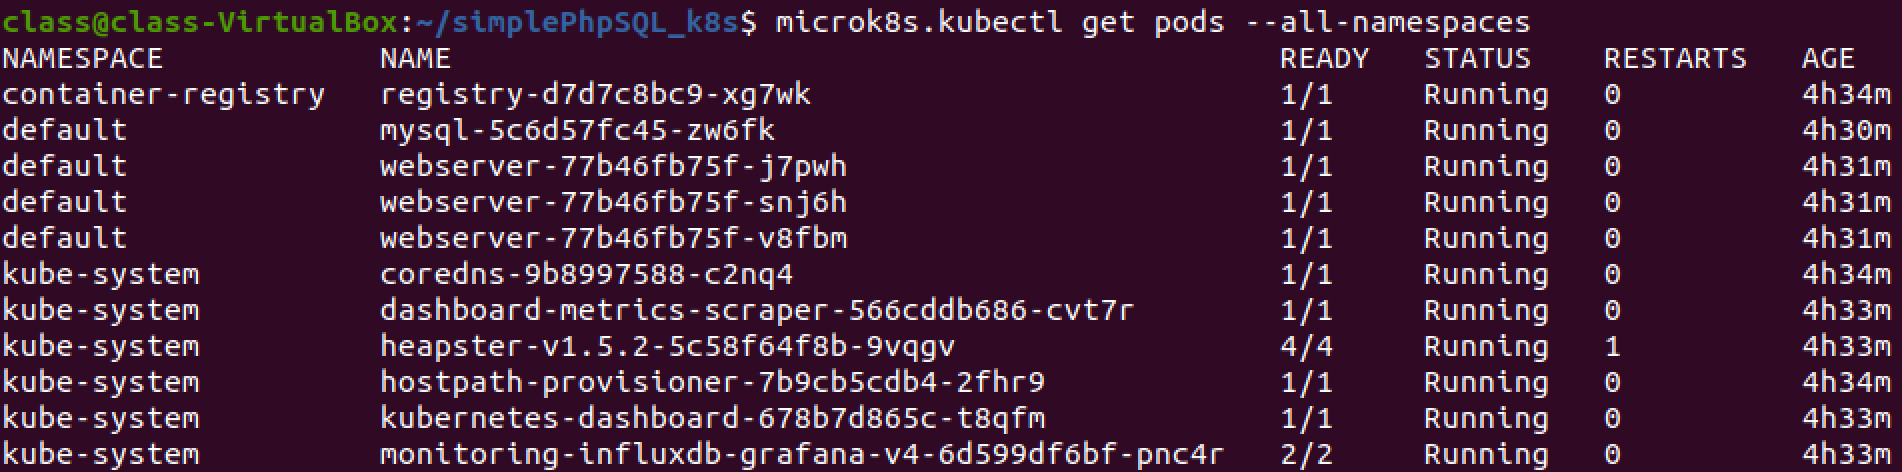
\includegraphics[width=1\linewidth]{./get_pods_1.png}
  \caption{\label{fig:pods}
  Output of microk8s.kubectl get pods --all-namespaces}
\end{figure}
\begin{figure}[htbp]
  \centering
  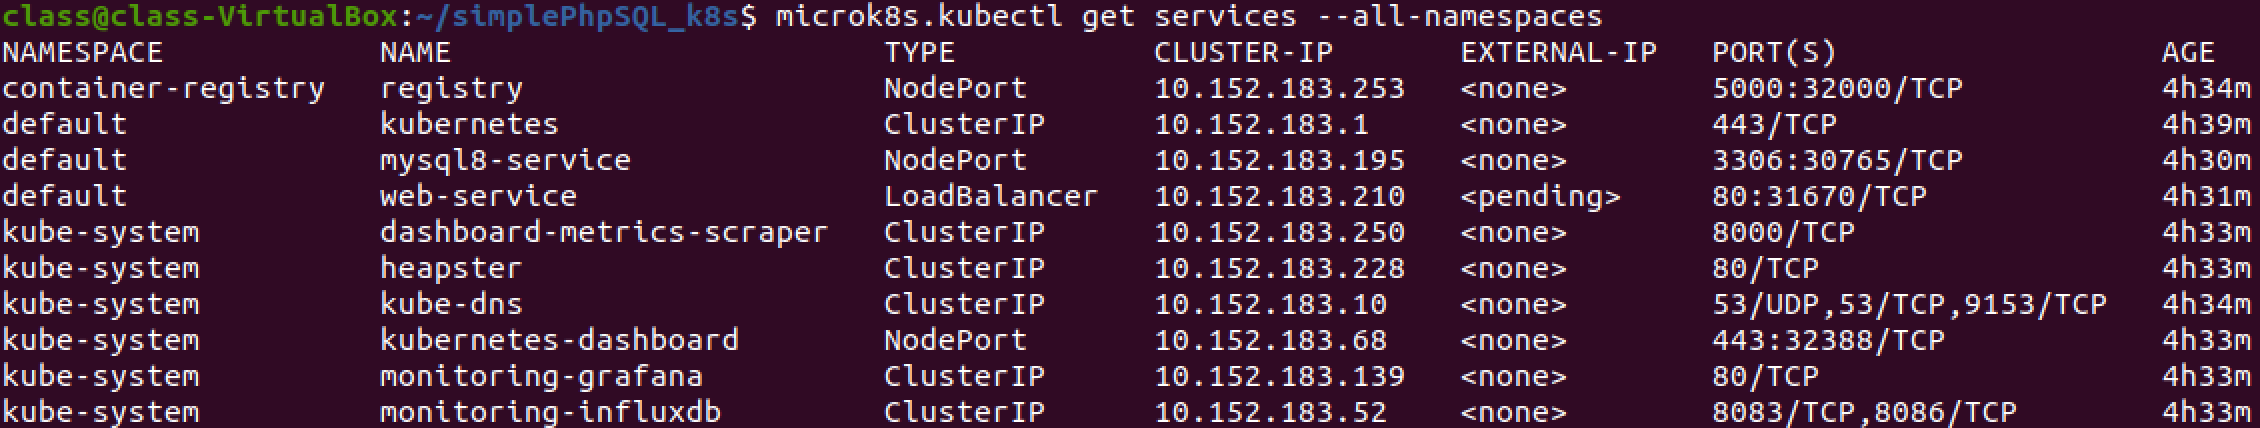
\includegraphics[width=1\linewidth]{./get_services_1.png}
  \caption{\label{fig:svcs}
  Output of microk8s.kubectl get services --all-namespaces}
\end{figure}
For example, the \verb|default| namespace refers to the default namespace for objects without any specified
namespace. Additionally, Kubernetes creates the \verb|kube-system| namespace, and it includes pods and services
like the dashboard.~\cite{namespace}\\
In the \verb|webserver.yaml| file, there are specifications on how many instances of each application to deploy
under \verb|spec/replicas|:
\begin{minted}{yaml}
  apiVersion: apps/v1
  kind: Deployment
  ...
  spec:
    replicas: 3
  ...
\end{minted}
This value can be changed to change the number of instances of web-servers. For example, if it was changed to 2,
then the output of the \verb|microk8s.kubectl get| commands would be the following:
\begin{figure}[htbp]
  \centering
  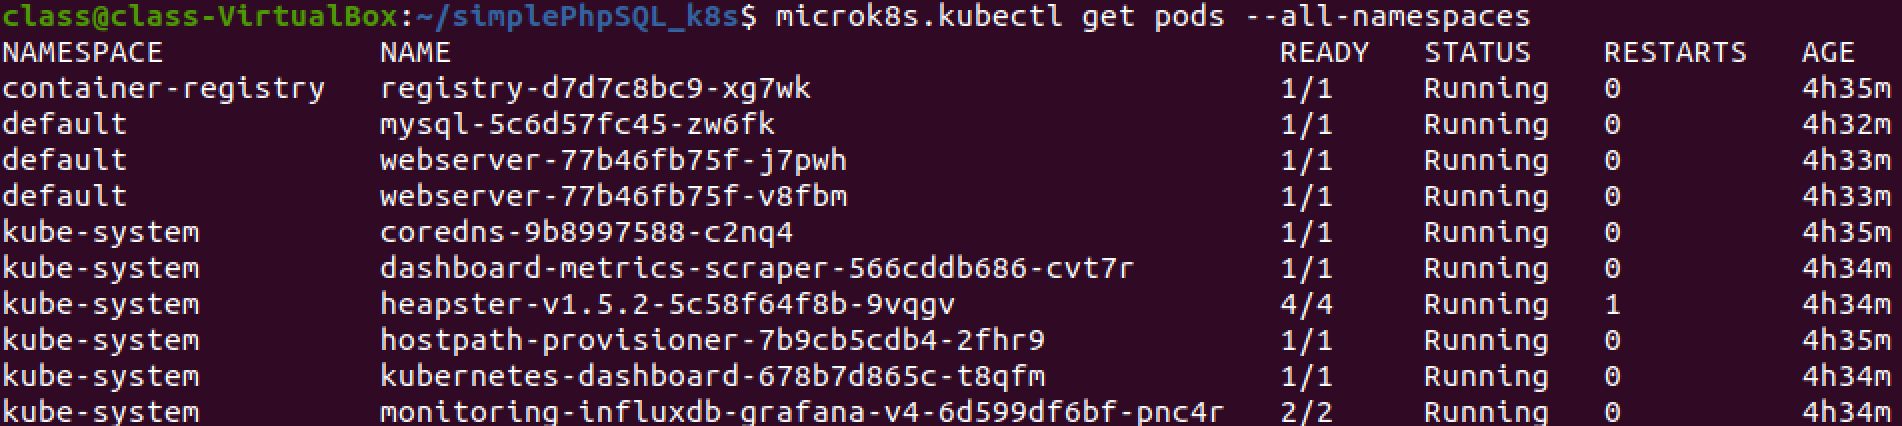
\includegraphics[width=1\linewidth]{./get_pods_2.png}
  \caption{\label{fig:pods2}
  New output of microk8s.kubectl get pods --all-namespaces}
\end{figure}
\begin{figure}[htbp]
  \centering
  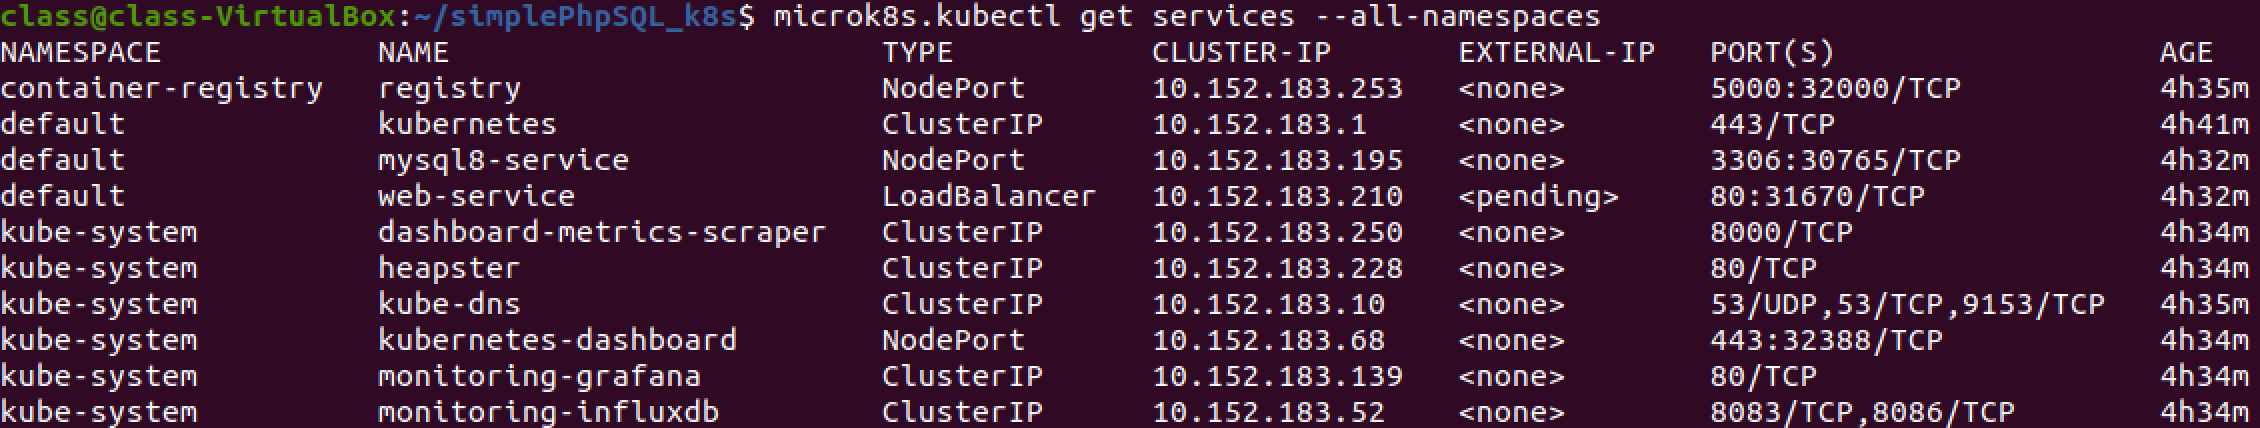
\includegraphics[width=1\linewidth]{./get_services_2.png}
  \caption{\label{fig:svcs2}
  New output of microk8s.kubectl get services --all-namespaces}
\end{figure}
\subsubsection*{RBAC}
For Role Based Access Control, first a service account and role need to be created and then
bound together. Then, the following command can be used to set up and run the Kubernetes
Dashboard:
\begin{minted}{bash}
  $ microk8s.kubectl -n kube-system
      edit service kubernetes-dashboard
\end{minted}
The type must be changed to \verb|NodePort| and the exposed port is given under \verb|ports/nodePort|:
\begin{minted}{yaml}
  ...
  spec:
    clusterIP: 10.152.183.68
    ports:
    - nodePort: 32388 # port num
      port: 443
      protocol: TCP
      targetPort: 8443
    selector:
      k8s-app: kubernetes-dashboard
    sessionAffinity: None
    type: NodePort # change from ClusterIP to NodePort
  ...
\end{minted}
Then, once a secret token is obtained, the dashboard can be opened and a list of all the pods in the
default namespace can be seen, like in Figure~\ref{fig:def_dash}. Only these pods are shown because
the namespace of the user-sa account is set to default, which is specified in the
\verb|sa-role-bind.yaml| file:
\begin{minted}{yaml}
  ...
  subjects:
  - kind: ServiceAccount
    name: user-sa
    namespace: default
  ...
\end{minted}
In order to create another service account that can access just the kube-system namespace, a new
service account must be initialized. This can be done by first creating a service account and then
making slight modifications to the \verb|user-role.yaml| and \verb|sa-role-bind.yaml| files, as can
be seen in \verb|part3/kube-role.yaml| and \verb|part3/kube-sa-role-bind.yaml|, respectively. After
creating the new service account, login to the dashboard with the token for the new account and now
nothing can be seen in the \verb|default| namespace, but the pods in the \verb|kube-system| namespace
are now visible on the dashboard, as shown in Figure~\ref{fig:kube_dash}. The sequence of commands
to set this up are as follows:
\begin{minted}{bash}
  $ microk8s.kubectl create serviceaccount kube-sa --namespace kube-system
  $ microk8s.kubectl apply -f kube-role.yaml
  $ microk8s.kubectl apply -f kube-sa-role-bind.yaml
\end{minted}
\begin{figure}[htbp]
  \centering
  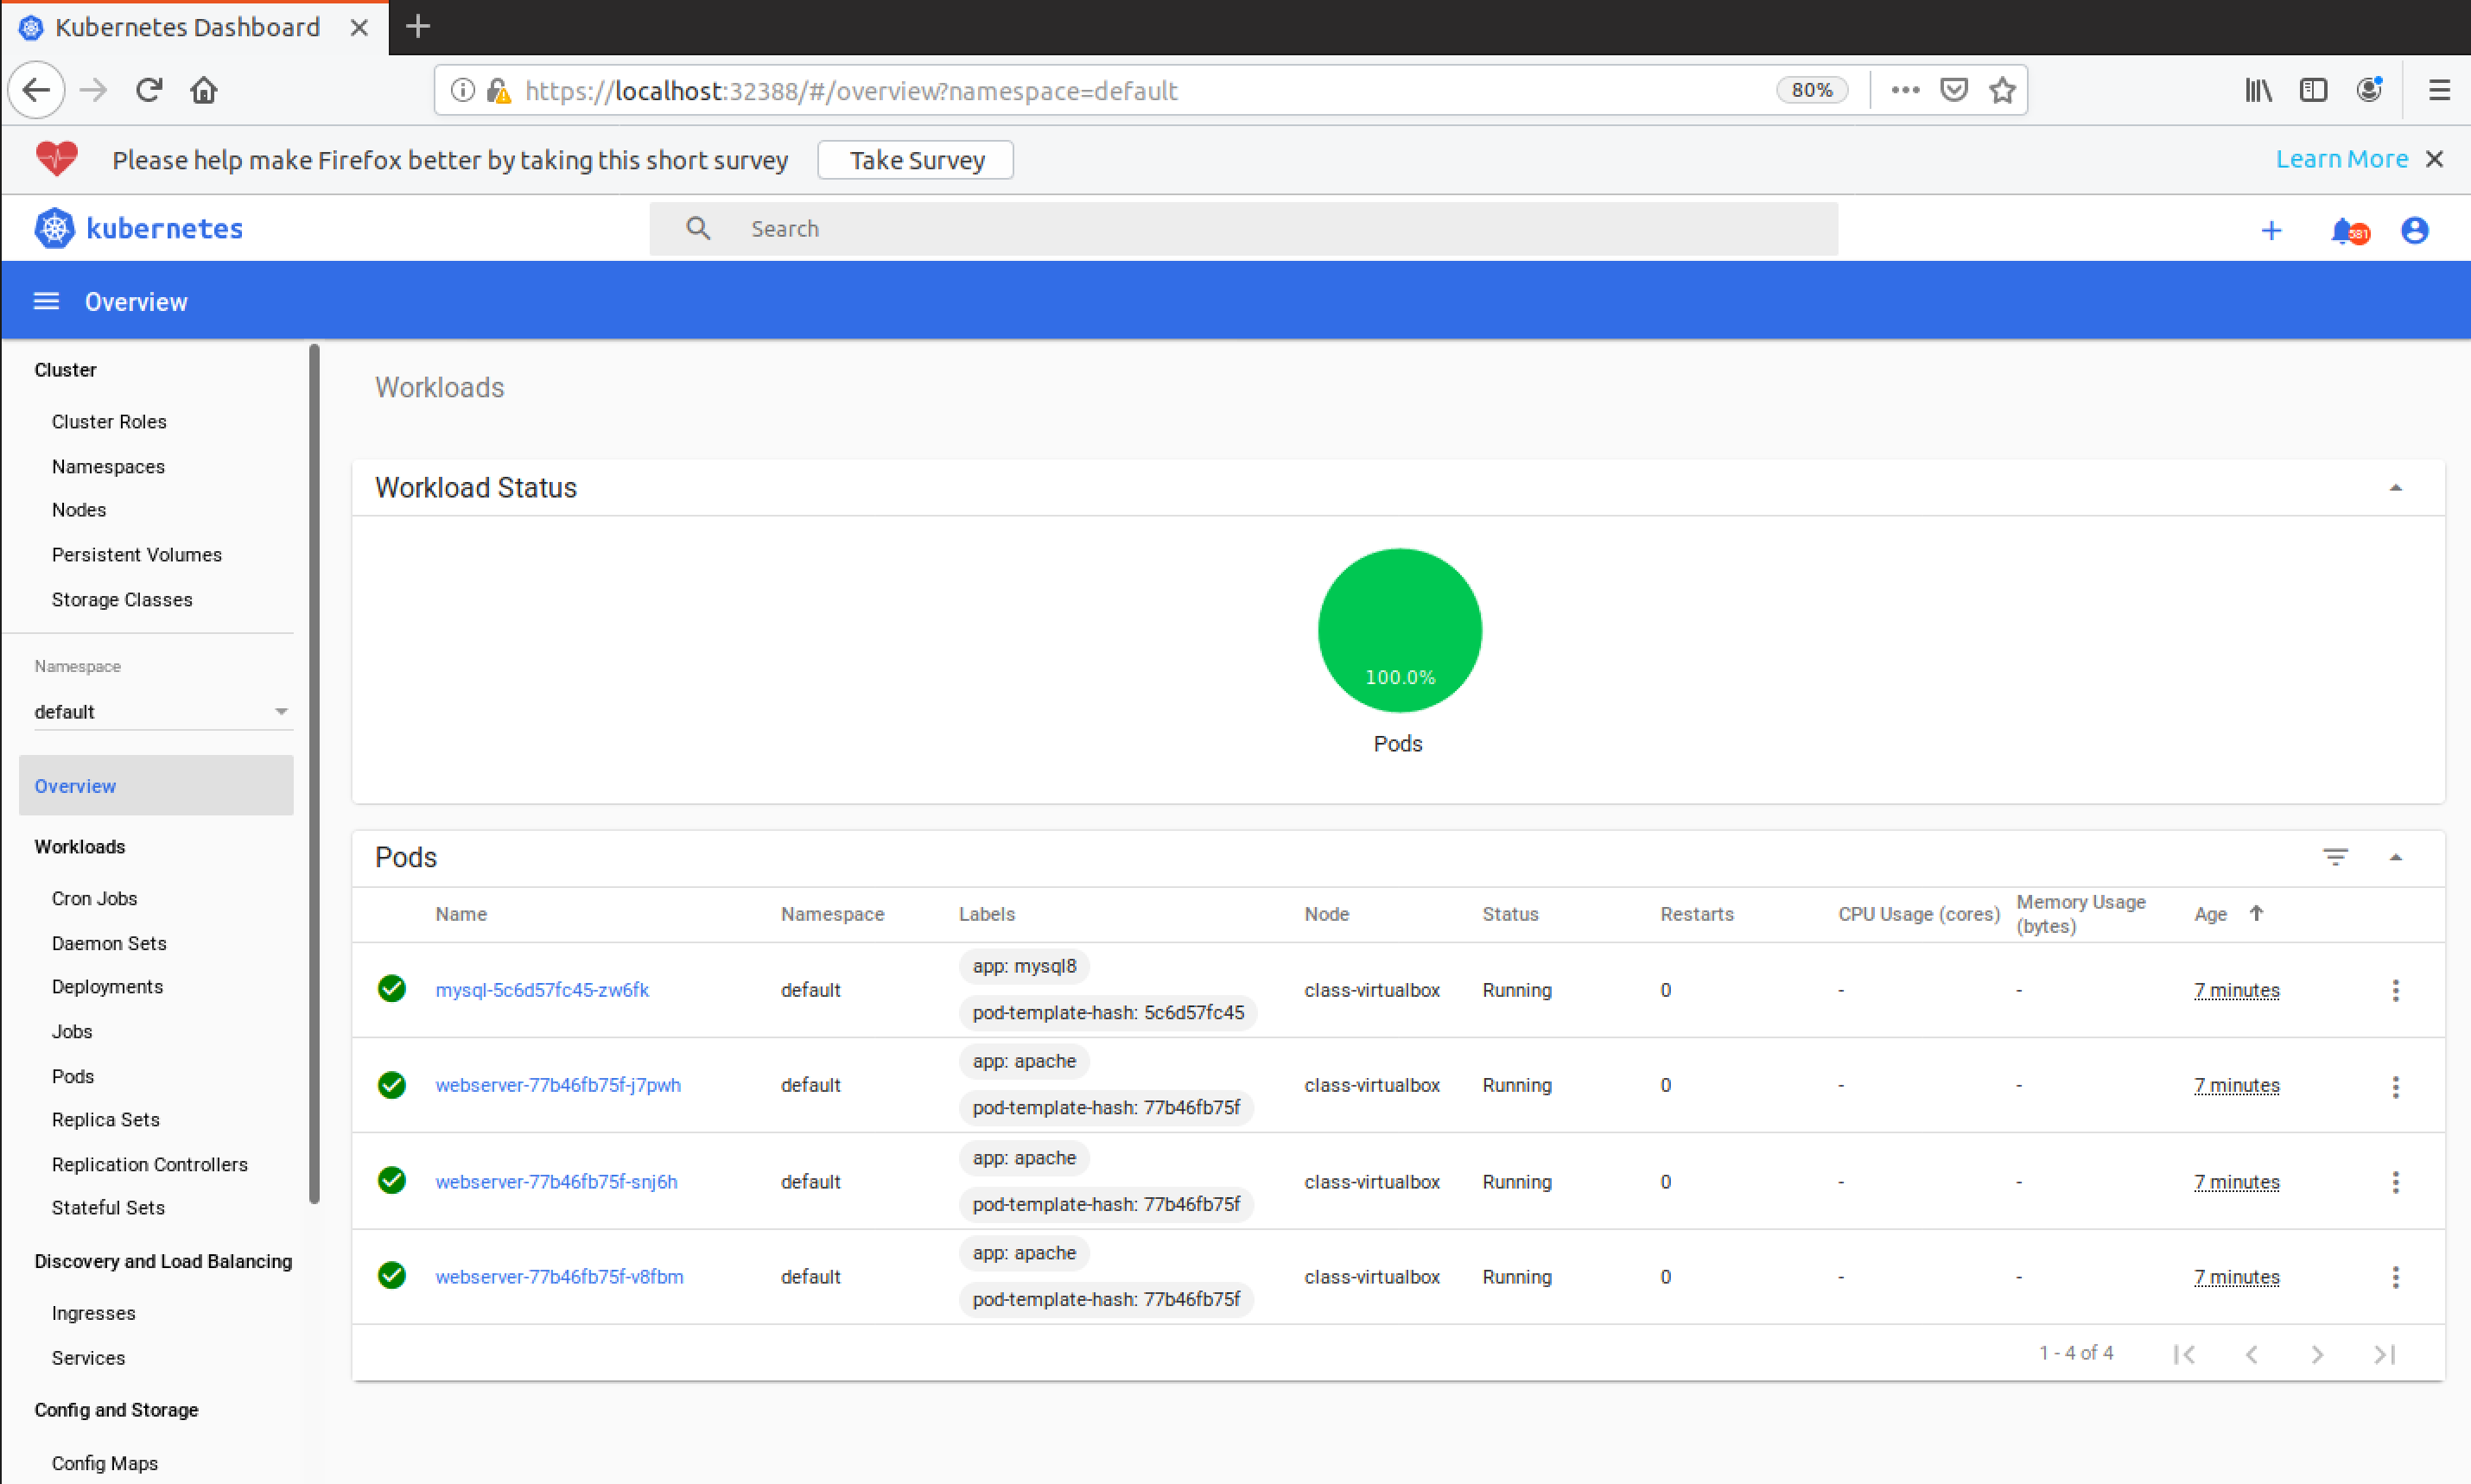
\includegraphics[width=1\linewidth]{./def_dash.png}
  \caption{\label{fig:def_dash}
  Dashboard view of default namespace visible to user-sa}
\end{figure}
\begin{figure}[htbp]
  \centering
  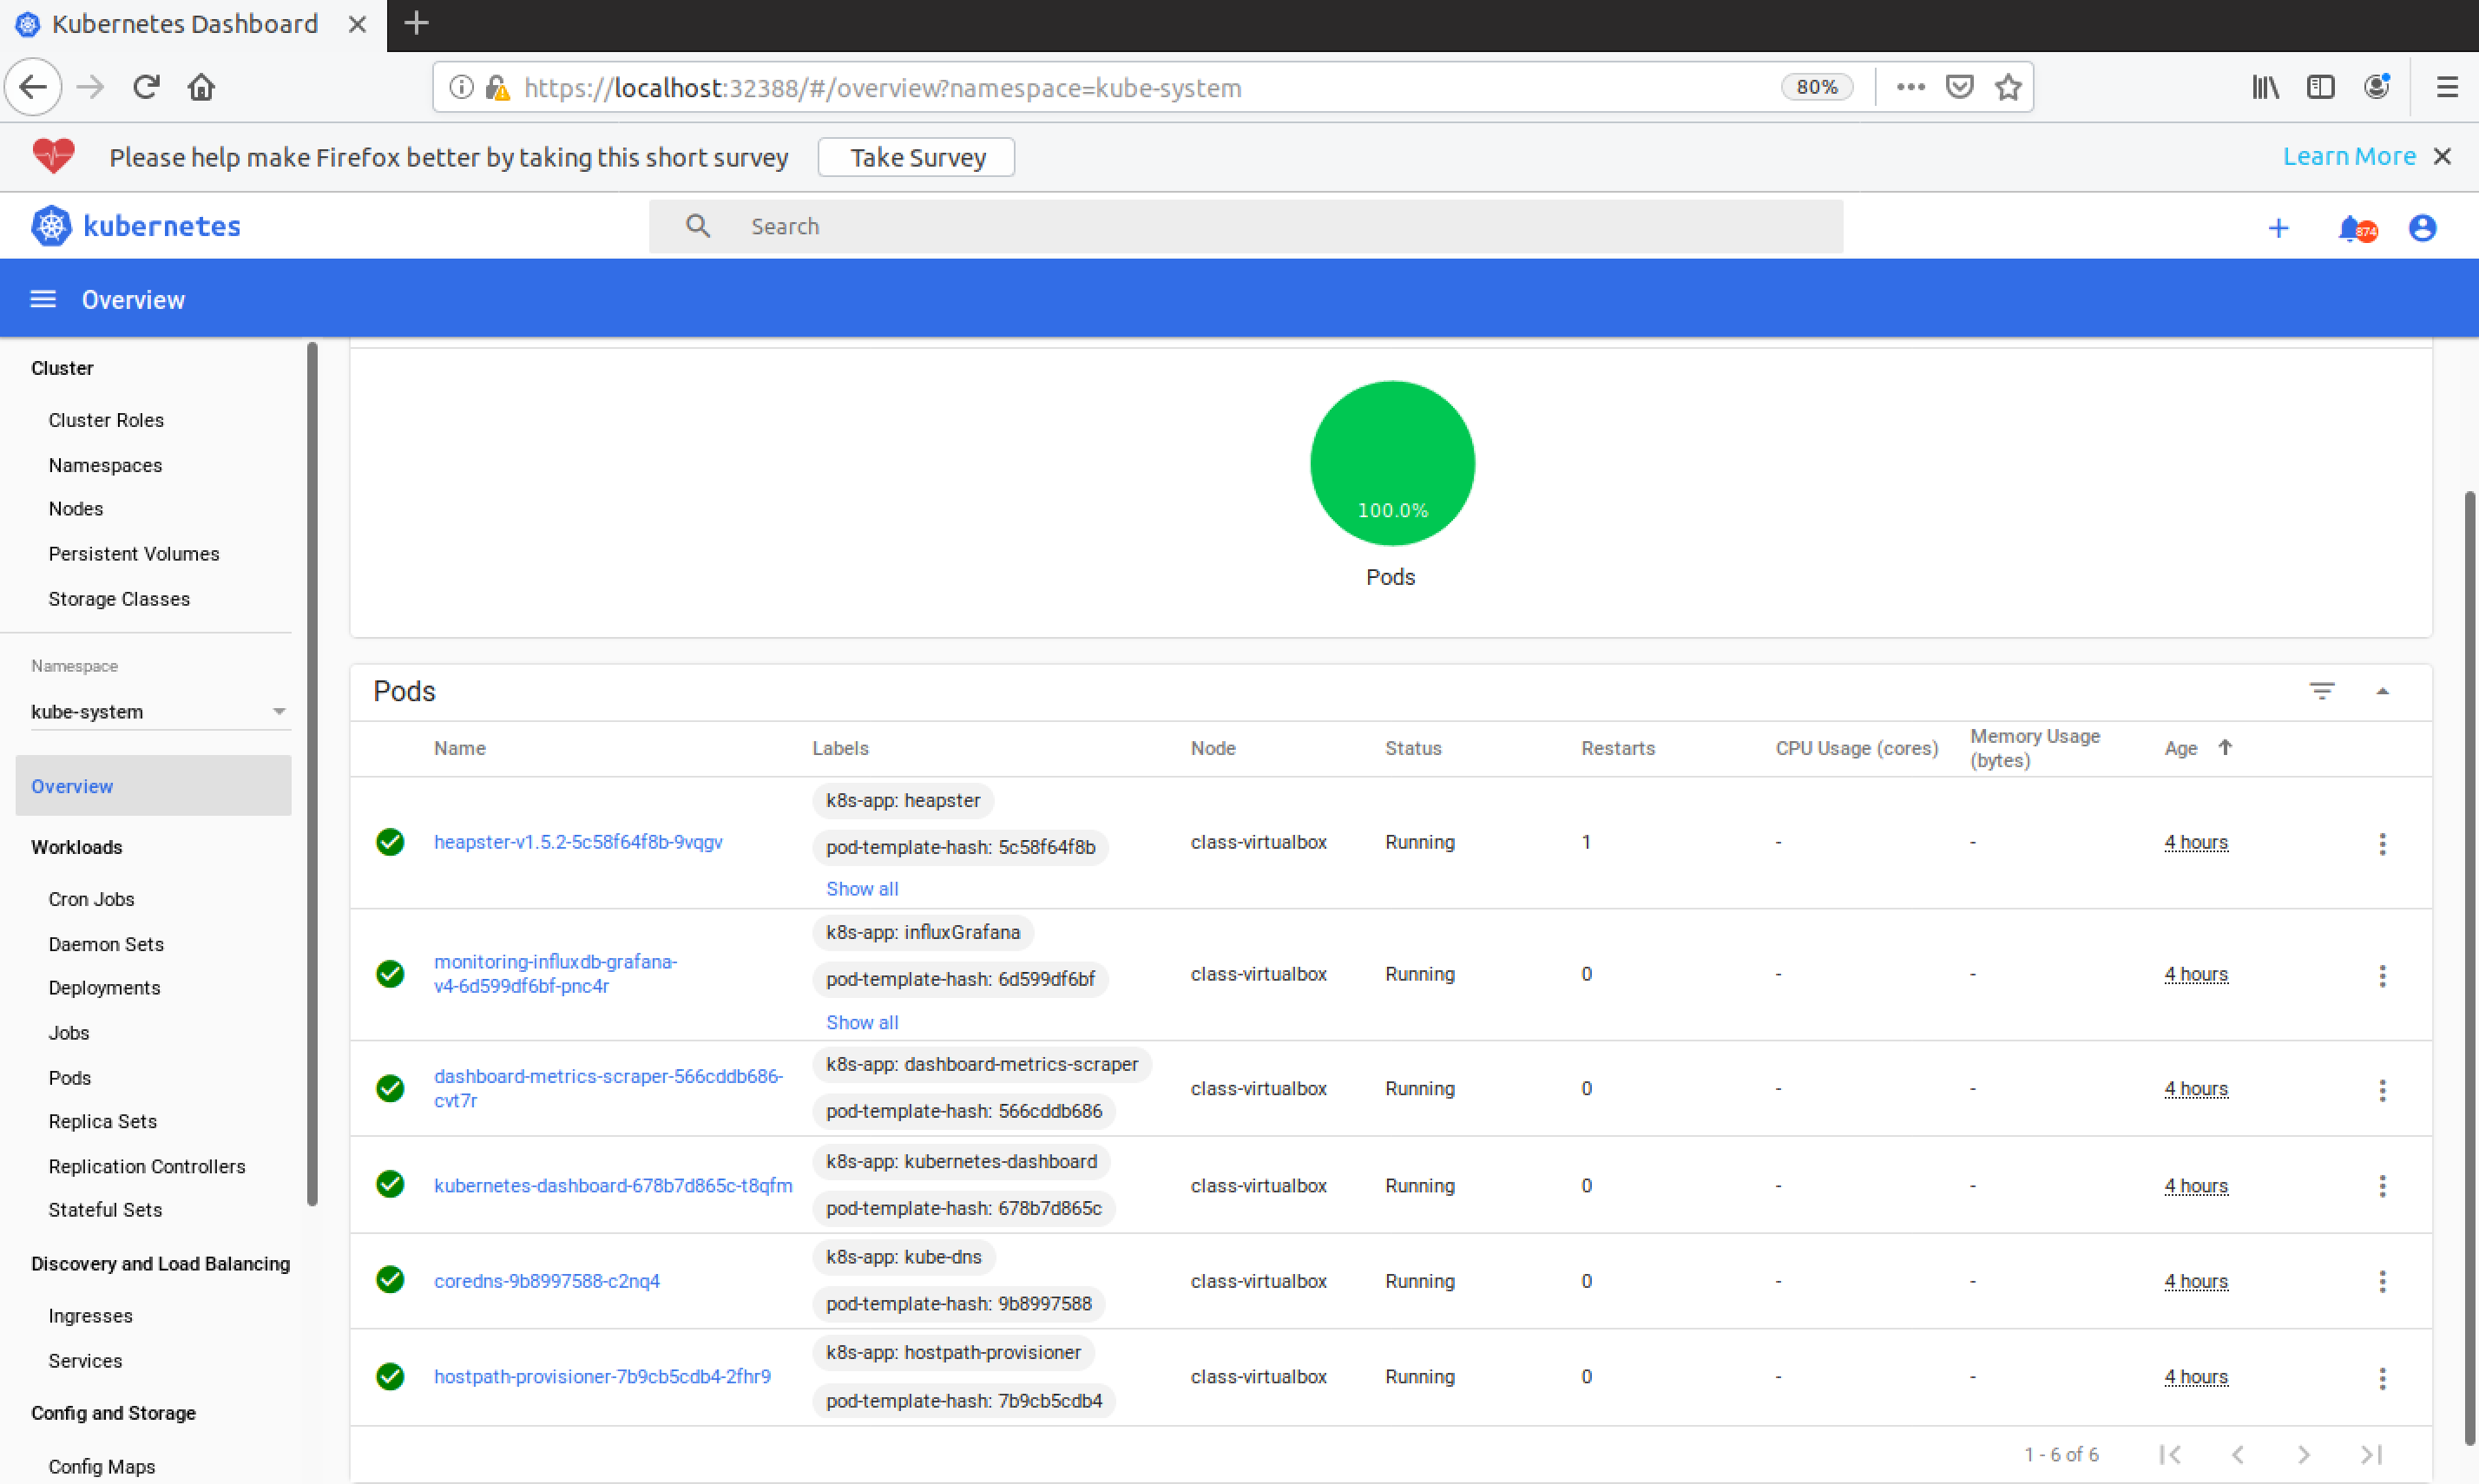
\includegraphics[width=1\linewidth]{./kube_dash.png}
  \caption{\label{fig:kube_dash}
  Dashboard view of kube-system namespace visible to kube-sa}
\end{figure}
\subsection*{3b - Creating a Kubernetes cluster for DVWA}
For this part, the Dockerfile for the Damn Vulnerable Web App was to be split into two, one for the
database and one for the web-app. The split Dockerfile and main.sh can be seen in \verb|part3/db/|
and \verb|part3/dvwa/|. Then, after the images are built, they needed to be deployed to Kubernetes.
After creating \verb|part3/mysql.yaml| and \verb|part3/webserver.yaml| by modifying the contents of
the corresponding files from the \verb|simplePhpSQL| project. The commands used to do this are:
\begin{minted}{bash}
  $ docker tag docker-vulnerable-dvwa_website:latest localhost:32000/docker-vulnerable-dvwa_website:k8s
  $ docker push localhost:32000/docker-vulnerable-dvwa_website:k8s
  $ docker apply -f mysql.yaml
  $ docker apply -f webserver.yaml
\end{minted}
Then, the pods can be seen in Figure~\ref{fig:split} with the resource consumptions as well.
\begin{figure}[htbp]
  \centering
  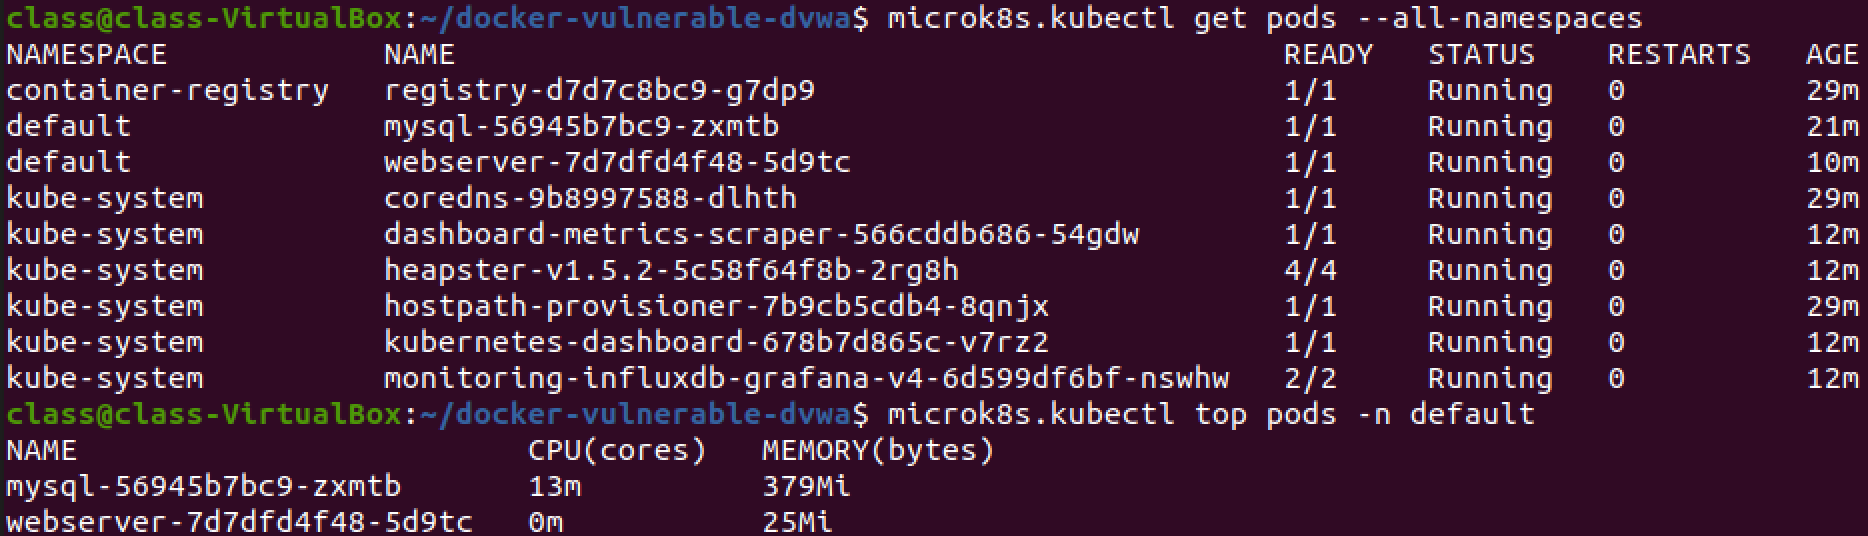
\includegraphics[width=1\linewidth]{./split_deploy.png}
  \caption{\label{fig:split}
  Pods and resource consumption of webserver after deploying the split DVWA}
\end{figure}
One issue is that the webserver could not connect to the database. The following are what
is believed to occur regarding the forkbomb injection.

If the script in \verb|part3/b.php| was injected into the web-app, it would crash the pod hosting
the web-app since it tries to run the fork bomb. In fact, without setting limits it seems to
crash the entire VM. This means that the website is not accessible until Kubernetes successfully
restarts it.\\ 
The web-app deployment can also be configured to launch multiple instances by changing the 
\verb|replicas| value in \verb|part3/webserver.yaml| to a number greater than 1 and redeploying it. 
Then, if the fork bomb
was run now, the application would have greater resiliency to it. In other words, given that
resource limitations have been set on the pods, the fork bomb would only take down one of the pods
while the others are still functional. Traffic is then redirected to the working pods while the
one that has crashed is terminated and brought up again. As a result, the website is still
accessible.\\
One DevOps use case for for Kubernetes is providing resiliency to these kinds of attacks so that
it becomes much harder to completely take down the service. Having multiple instances also means
that one pod can be upgraded and deployed without having to take down the whole service. Then the
pod(s) that haven't been upgraded can be done with little to no downtime. Another usage is that
having mutliple instances can better balance heavy loads and make full use of the host's resources.
\section*{Conclusion}
There were lots of strange issues that were very difficult to troubleshoot, making this lab
frustrating and time consuming. It provided a good, hands-on way to explore the material,
but it was difficult to figure out exactly how to divide the DVWA into two images and connect them
after deploying to Kubernetes. Besides that difficulty with Docker, this lab helped with learning
more about Kubernetes.
\bibliography{bibliography}
\bibliographystyle{ieeetr}
\end{document}
